\documentclass[12pt]{article}
\usepackage[latin9]{inputenc}
\usepackage{array}
\usepackage{float}
\usepackage{amsmath}
\usepackage{graphicx}
\usepackage[authoryear]{natbib}
\usepackage[unicode=true]{hyperref}
\usepackage{breakurl}

\makeatletter

\oddsidemargin 0in \evensidemargin 0in \topmargin 0in \columnsep 10pt
\columnseprule 0pt \marginparwidth 90pt \marginparsep 11pt
\marginparpush 5pt \headheight 0pt \headsep 0pt \textheight 9in
\textwidth 6.5in

%\setlength{\voffset}{0.5in}
\usepackage{threeparttable}
\usepackage{setspace}
\usepackage{rotating}
\usepackage{amsthm}
\usepackage[usenames]{color}
%\usepackage{lscape}
\usepackage{appendix}
\usepackage{booktabs}
\usepackage{epstopdf}
\usepackage{tabularx}
\usepackage{longtable}

%Uncomment one of these to put figures at the end.
%\usepackage[nolists]{endfloat}

\usepackage{datetime2,datetime2-calc}
\DTMnewdatestyle{Myyyy}{%
  \renewcommand*{\DTMdisplaydate}[4]{\DTMmonthname{##2}~##1}%
  \renewcommand*{\DTMDisplaydate}{\DTMdisplaydate}%
}
\DTMsetdatestyle{Myyyy}

\usepackage{xcolor}
\hypersetup{
    colorlinks,
    linkcolor={blue!80!black},
    citecolor={blue!80!black},
    urlcolor={blue!80!black}
}

\usepackage[position=top]{subfig}
\captionsetup{position=top}

\@ifundefined{showcaptionsetup}{}{%
 \PassOptionsToPackage{caption=false}{subfig}}
\usepackage{subfig}
\makeatother

% DEFINING PATH TO FIGURES AND TABLES
\newcommand{\figpath}{../output/offline/figures}
\newcommand{\tablepath}{../output/offline/tables}

% SET FOOTNOTE SIZE AT 12pt
\renewcommand{\footnotesize}{\normalsize}

% DOUBLESPACE FOOTNOTES
\usepackage{footmisc}
\renewcommand{\footnotelayout}{\doublespacing}
\setlength{\footnotesep}{1.25\baselineskip}

\begin{document}

\doublespace

\title{Pass-Through of Own and Rival Cost Shocks: Evidence from the U.S. Fracking Boom\thanks{We thank Ryan Kellogg, Katheryn Russ, Joe Shapiro, Jim Stock, Reed Walker and seminar participants at Harvard, Duke, University of Connecticut, University of Maryland, the NBER Hydrocarbon Infrastructure and Transportation workshop, the Empirical Methods in Energy Economics workshop, and Berkeley Energy Camp for helpful comments. Both authors declare they have no interests, financial or otherwise, that relate to the research described in this paper, nor do they have any current ties, directly or indirectly to the energy industry. This work has been supported by the Sloan Foundation and NBER Hydrocarbon Infrastructure and Transportation workshop. Assistance with the data from the Energy Information Administration, especially Joseph Conklin and Lawrence Stroud, is gratefully acknowledged. }}

\author{Erich Muehlegger \thanks{University of California - Davis and NBER, \protect\href{mailto:emuehlegger@ucdavis.edu}{emuehlegger@ucdavis.edu}.} \\
 Richard L. Sweeney \thanks{Boston College, \protect\href{mailto:sweeneri@bc.edu}{sweeneri@bc.edu}.}}

\date{\today \\
 \textbf{}}
\maketitle

\begin{abstract}
\normalsize
In imperfectly competitive settings, a firm's price depends on its own costs as well as those of its competitors. We demonstrate that this has important implications for the estimation and interpretation of pass-through. Leveraging a large input cost shock resulting from the fracking boom, we isolate price responses to firm-specific, regional and industry-wide input cost shocks in the US oil refining industry. The pass-through of these components vary from near zero to full pass-through, reconciling seemingly disparate results from the literature. We illustrate the policy implications of rival cost pass-through in the context of a tax on refinery carbon emissions.

\bigskip{}

JEL Codes: H22, H23, Q40, Q54

\bigskip{}
\end{abstract}
\setcounter{page}{1}

\clearpage

\section{Introduction}

Pass-through of taxes or input costs onto prices is a central policy parameter with wide ranging economic implications. Pass-through is used to estimate the incidence of actual taxes (e.g., \citet{marion_fuel_2011,fabra_pass-through_2014,stolper_who_2016}), the distributional impacts of trade tariffs (e.g., \citet{amiti2019impact,fajgelbaum2019return}), the beneficiaries of major entitlement program subsidies (e.g., \citet{duggan2016benefits}), and to forecast the incidence of hypothetical taxes (e.g., \citet{ganapati_incidence_2017}). It is used as a sufficient statistic for welfare analysis (e.g., \citet{chetty_sufficient_2009}) and to recover other objects of economic importance, such as trade costs (\citet{atkin_whos_2015}), international propagation of inflation shocks (\citet{gopinath2008sticky,auer2017international} or demand elasticities (\citet{miller_using_2013}).

In this paper, we demonstrate that the nature of the tax or input cost shock used to estimate pass-through is \emph{directly} related to the pass-through rate recovered. In oligopolistic settings, the price a firm sets depends directly on its own costs, but also indirectly on its rivals' costs. This simple observation has two important implications for pass-through analysis. First, when estimating a firm's response to a change in its own costs, it is important to account for rival responses as well. Beyond simple omitted variable bias from correlated cost shocks, the strategic response of seemingly untreated firms to rival cost changes invalidates them as a control group.\footnote{The empirical pass-through literature rarely incorporates the indirect effects of competitors' cost changes explicitly. Instead, papers often consider the robustness of estimates by limiting the control group to the most distant ``untreated'' firms. As examples, \citet{dube2010minimum} uses interior rather than border counties when estimating the effect of minimum-wage laws.  \citet{fowlie2012emissions} considers geographically distant and unaffiliated facilities when examining the impacts of the RECLAIM program.} Second, when using pass-through for policy prediction, the identifying variation used in estimation must match the policy application. For example, a pass-through estimate identified from firm-level cost or tax shocks may substantially underestimate the price impact of an industry-wide policy change.

We demonstrate these points empirically by studying the response of prices in the U.S. oil refining industry to large input cost shocks resulting from the fracking boom. Our setting allows us to overcome three challenges that have limited the consideration of rival cost pass-through in past papers: (1) the need for comprehensive input and output prices for the universe of firms, (2) the ability to observe which firms are direct competitors, and (3) an exogenous input cost shock that differentially affects firms.  We examine restricted-use microdata on the universe of oil refiners in the United States from the Energy Information Administration.  For each firm, we observe crude oil procurement costs, detailed plant-level production decisions, and monthly prices and quantities sold for all refined products at the state-level. Such rich firm-level data on production, input and output prices are rarely available.\footnote{\citet{fabra_pass-through_2014} is a notable exception, examining bids and carbon intensities for the universe of Spanish electricity generators.}  The confidential sales data allow us to incorporate the spatial supply patterns of the industry directly, rather than make assumptions about which firms directly compete.\footnote{\citet{miller_pass-through_2017} also studies rival cost pass-through, documenting more-than-full pass-through of energy prices in the Portland cement industry, but does not observe firm-specific prices nor which firms directly compete.} Finally, our data span the U.S. fracking boom, which led to a near doubling of U.S. oil production between 2008 and 2015. Despite the scale of the shock, a set of regulatory, logistical and technological constraints limited the extent to which some refineries could benefit. The net result was a large reduction in oil input costs of some refiners, while the costs of other firms, producing identical products and often located nearby, remained largely unchanged.

The heterogenous impact of this cost shock allows us to separately identify the response to refiners' own-costs, their direct competitors' costs, and industry-wide cost shocks.\footnote{Sharing the spirit of this exercise, \citet{amiti2018much} illustrates the importance of decomposing firm-borrowing and bank-supply shocks as drivers of firm investment and \citet{amiti2018international} examines strategic complementarity in price setting amongst manufacturing firms.}  We estimate pass-through rates that vary from near zero, for firm-specific shocks, to full, for industry-wide shocks. Viewed as a continuum, these estimates reconcile seemingly conflicting pass-through estimates from the recent fuel pass-through literature.  Using regional variation in energy prices, \citet{ganapati_incidence_2017} finds refineries are largely unable to pass-through costs; while using national variation in the cost of renewable fuel credits, \citet{knittel_pass-through_2017} and \citet{lade_jaere_2019} finds that the incidence falls fully on consumers.\footnote{Similar results on full pass-through are obtained in the transmission of state fuel taxes (e.g., \citet{doyle_jr._$2.00_2008}, \citet{marion_fuel_2011}, and \citet{stolper_who_2016}))} We interpret the disconnect in these estimates as reflective of the distinction between idiosyncratic and shared cost variation, and show analytically that price changes will naturally vary for these two shocks, even after conditioning on a firm's own costs.

We conclude by demonstrating the relevance of these results for policy analysis. We consider a hypothetical carbon tax on refineries, the second largest industrial point-source of emissions in the U.S.  When paired with a border adjustment tax, a carbon tax is equivalent to an industry-wide cost shock.  Properly accounting for the indirect effects of competitors, our results suggest consumers  bear virtually all of the tax.  Moreover, 45 percent of firms, which are relatively less carbon-intensive than their rivals, more than fully pass-on an industry-wide carbon tax. Yet, an estimate of tax pass-through based on within market-time variation in costs would suggest prices rise by a mere five cents per dollar of tax imposed. This exercise highlights the importance of matching the cost variation used to estimate pass-through with the scope of the policy to which the estimate is applied.

\section{Pass-through and Imperfect Competition\label{sec:Pass-through}}

A long-standing theoretical literature studies pass-through in imperfectly competitive markets.  \citet{bulow_note_1983} and \citet{fevrier_idiosyncratic_2004} consider pass-through in Bertrand and Cournot markets, illustrating the possibility that pass-through can exceed one in oligopolistic markets; \citet{weyl_pass-through_2013} provide a more general framework.  Similar links between pass-through and competition arise in the pricing-to-market literature (e.g.,  \citet{bernard2003plants,atkeson2008pricing,de2015understanding, amiti2018international}) wherein endogenous firm-level markups are an outcome of the competitive environment.  We draw upon these papers to illustrate how pass-through relates to the scope of a cost shock (that is whether a cost shock affects a single firm or a firm and its rivals), and to highlight the importance of accounting for competitor costs in empirical estimation.

Here, we consider the pass-through ($\rho$) of a tax ($\tau$) onto the price of firm $i$, although an input cost shock, like the oil price shock we study, could be considered analogously.  For expositional simplicity, we consider competition in prices, although we present examples for other models competition in Appendix A.  Firm $i$ sets profit-maximizing price $p_i$ and faces marginal costs inclusive of taxes of $\alpha_i$. We allow each firm to be differentially exposed to the tax, with $\frac{\partial \alpha_i}{\partial \tau}$ capturing the marginal per-unit tax rate faced by firm $i$.\footnote{In our empirical context, variation in exposure arises from differential access to low-cost crude oil and in our policy exercise, from differential carbon-intensity of production.}  Formally, we decompose the pass-through of the tax onto firm $i$'s price as a direct effect and an indirect effect operating through $i$'s competitors:

\begin{equation}
\rho_i(\tau)=\frac{\partial p_i}{\partial\alpha_i}\frac{\partial \alpha_i}{\partial \tau} + \sum_{j \neq i} \left[\frac{\partial p_i}{\partial p_j} \frac{\partial p_j}{\partial\alpha_j}\frac{\partial\bar{\alpha}}{\partial \tau}+\frac{\partial p_i}{\partial p_j}\frac{\partial p_j}{\partial\alpha_j}(\frac{\partial\alpha_j}{\partial \tau} - \frac{\partial\bar{\alpha}}{\partial \tau})\right]
\label{eq: MS_passthrough}
\end{equation}
where $\frac{\partial \bar{\alpha}}{\partial \tau}$ is the average marginal tax rate, and $\frac{\partial p_i}{\partial p_j}$ reflects firm $i$'s optimal response to a change in firm $j$'s price.

A tax affects a firm's choice of strategy both \textit{directly}, through the firm's own costs, and \textit{indirectly}, in response to the strategic choice of the firm's competitors. Thus, a tax borne by the firm \emph{alone} will be passed-through at a different rate than a tax affecting the firm and its competitors.  We further decompose the indirect effect into two components - the effect of the mean shock to the firm's competitors and the competitor-specific deviation from the shock, reflected in the second and third terms of equation (\ref{eq: MS_passthrough}).  If firm $i$'s competitors face different tax exposure, pass-through depends on the covariance between relative exposure $(\frac{\partial \alpha_j}{\partial \tau} - \frac{\partial \bar{\alpha}}{\partial \tau})$ and the degree to which firms $i$ and $j$ are close rivals, $\frac{\partial p_{i}}{\partial p_{j}}$.  If a firm's closest rivals are more heavily impacted by a tax, the firm can pass-through their shock to a greater degree.

These results have three implications relevant to the estimation and interpretation of pass-through. First, omitting shocks to rival firms will bias own-cost pass-through estimates if shocks are correlated across firms.\footnote{\citet{pennings2017pass} notes a similar bias if real exchange rate shocks are correlated across countries.} Second, firms which are not directly affected by a shock may still adjust their prices if their rivals are affected. This behavior violates the stable unit treatment value assumption implicit in common estimation strategies, which use the price of rivals not directly affected by a cost shock as contemporaneous counterfactual. Finally, empirical pass-through rates are specific to the identifying variation used for estimation. Even after conditioning on the shock faced by a firm, the resulting price change will vary depending on whether that shock affects only the firm or is shared by its rivals as well. To compute the full price response to a cost shock or policy change, it is necessary to incorporate both the direct and indirect effects. However, empirical models that rely on rich temporal or spatial fixed effects may subsume the latter.  This constrains the econometrician to estimating the pass-through rate of a firm-specific shock, which may or may not be of primary policy interest. We illustrate each of these points in our empirical results.

\section{Empirical Setting and Institutional Details \label{sec:Background}}

Oil refineries process crude oil into refined end-products like gasoline and diesel. Although the United States imports substantial amounts of crude oil, U.S. refineries produce almost all end-products consumed domestically. Most U.S. refineries are located proximate to traditional oil deposits, such as Texas, Louisiana and California, rather than areas that demand refined fuels.\footnote{Appendix Figure B.1 maps refineries by capacity.}   The industry relies heavily on pipelines to move crude oil to refineries and to ship refined products to demand centers. These pipeline networks dictate both the locations from which refineries can cheaply acquire crude and end markets to which refiners can competitively ship.  Despite this spatial mismatch of supply and demand, entry is limited - no new refineries have been built since the early 1980's.

\subsection{Data \label{sec:Data}}

Through a confidential data request, we obtained data on refinery operations from the Energy Information Administration, described in detail in appendix Table B.1. A key feature of the EIA data is that we directly observe output prices and crude input costs (which account for over 90\% of variable costs), allowing us to directly observe margins for each firm. Every firm that owns a refinery in the United States reports the total volume and cost of crude oil acquired both domestically and abroad each month, by Petroleum Administration Defense District (PADD).\footnote{PADD's are a commonly used geographic aggregation for the industry dating back to World War II. For a map, see appendix Figure B.1.} These firms also report detailed monthly production data at the \emph{refinery} level, including the quality of crude oil used. On an annual basis, they also report operable capacity and exhaustive information on the technology installed. Finally, at the \emph{state} level, each firm reports the monthly volume sold and average price of all end products, broken out by sales to end users (retail) and sales for resale (wholesale).\footnote{Where a firm owns multiple refineries in a PADD, we assume that the firm supplies states from the refinery with the lowest transportation costs, described further in appendix B.2.} The sample in which all surveys are observed spans 2004-2015, and the resulting 9,215 firm-PADD-month observations are summarized in appendix Table B.3.

\subsection{Fracking background \label{sec:Fracking}}

The EIA data spans the U.S. fracking boom, which is the source of our input cost shock. Shortly after the turn of the century, two complementary technologies, hydraulic fracturing and horizontal drilling, rapidly matured, unlocking trillions of dollars of previously uneconomical domestic oil reserves. The ensuing transformation of the U.S. oil industry is documented in the four panels of Figure \ref{fig4}.

U.S. crude oil production nearly doubled between 2008 and 2015, abruptly reversing a decades-long trend towards the use of imported oil (Figure \ref{fig4}\hspace{-1pt}\subref*{fig4:USProd}).  As a consequence, a previously superfluous 1977 ban on the export of crude oil became binding, and U.S. crude oil spot prices diverged from international crude markets (Figure \ref{fig4}\hspace{-1pt}\subref*{fig4:WTI}). At the start of the boom, from 2010 to 2015, the West Texas Intermediate (``WTI'') spot price averaged \$12 per barrel below the Brent spot price, in comparison to trading at an average \$1.41 per barrel premium from 2000 to 2010.

\begin{figure}%
  \centering
  \caption{Shale Boom and U.S. Refining \label{fig4}}
  \subfloat[U.S. Oil Production]{\includegraphics[width=0.48\textwidth]{\figpath/from_public_data/mono_EIA_oil_production_PADD.png} \label{fig4:USProd}}
  \hspace{5pt}%s
  \subfloat[U.S. vs Global Spot Prices]{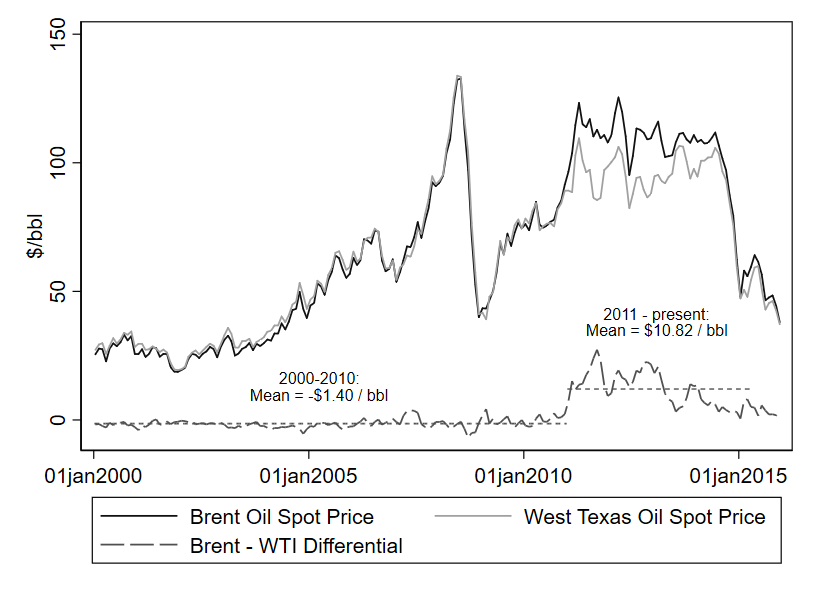
\includegraphics[width=0.48\textwidth]{\figpath/from_public_data/mono_oil_spot_price.png} \label{fig4:WTI}}\\
  \subfloat[Regional Input Cost Differential]{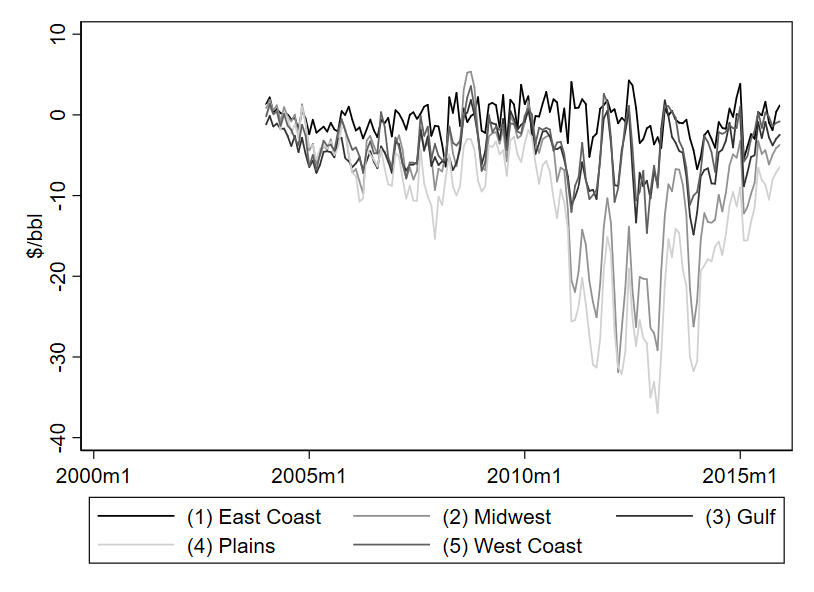
\includegraphics[width=0.48\textwidth]{\figpath/from_public_data/mono_EIA_PADD_price_diff_brent.png} \label{fig4:PADD_diff}}
  \hspace{5pt}%s
  \subfloat[Domestic Light-Heavy Crude Spread]{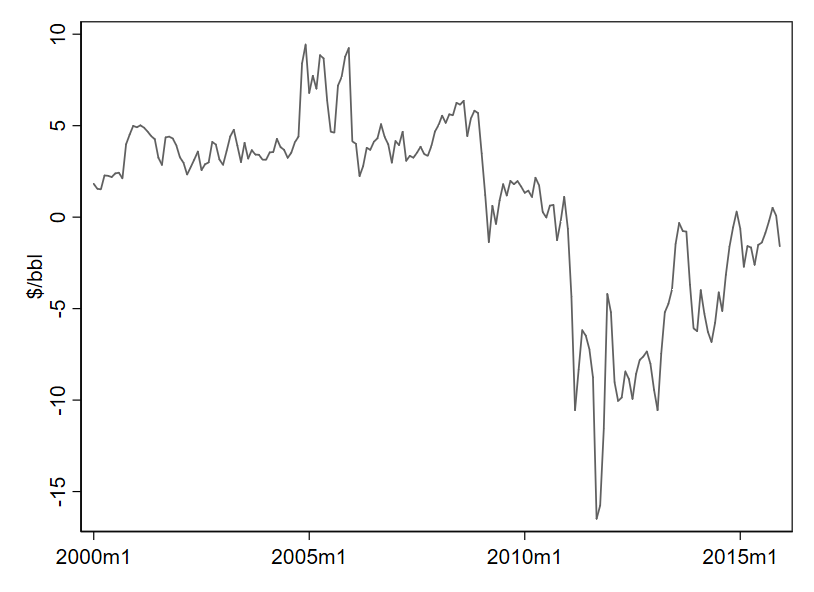
\includegraphics[width=0.48\textwidth]{\figpath/from_public_data/mono_DomFPP_HL_spread_4020.png} \label{fig4:API_diff}} \\
  \begin{minipage}{.9\linewidth} \doublespacing
  Description: \subref{fig4:USProd} U.S. oil production by PADD;
  \subref{fig4:WTI} West Texas Intermediate (WTI) and Brent spot prices;
  \subref{fig4:PADD_diff} Average crude price paid by refiners, minus the contemporaneous Brent spot price, by PADD (PADD-level data only available beginning in 2004); and,
  \subref{fig4:API_diff} U.S. light - heavy crude spread, as approximated by the difference between the average price for crudes with API gravity between 35 and 40, minus the average price for crudes with API gravity between 20 and 25.
  \end{minipage}
\end{figure}

Within the United States, the gains from the fracking boom were not equally shared among refiners. The most productive shale plays were in the middle of the country, while domestic production elsewhere continued to decline (Figure \ref{fig4}\hspace{-1pt}\subref*{fig4:USProd}). In the Gulf Coast, shale oil was proximate to major conventional oil fields, the largest concentration of refineries, and the epicenter of the crude distribution system. But in the Midwest, primarily North Dakota, relatively little pipeline capacity existed to move ``tight'' oil from shale fields to refineries. As a result, refineries in the Rocky Mountains (PADD 4) and Midwest (PADD 2) could acquire crude oil at a significant discounts, while crude costs for coastal refineries tracked foreign markets more closely (Figure \ref{fig4}\hspace{-1pt}\subref*{fig4:PADD_diff}).

Within region, some refiners were better positioned to benefit from the boom than others, due to the attributes of shale oil. Crude oil is highly differentiated, and refineries are finely tuned to process specific types of crude oil. The most important dimension along which crudes are differentiated is density. Dense crudes (measured by a low API gravity) require more processing,  more sophisticated capital, and typically trade at a discount relative to ``lighter'' crudes.  But, the oil produced from the most active shale plays in the United States has been very light (high API gravity).  The boom in light oil production reversed the historical correlation between price and crude density (Figure \ref{fig4}\hspace{-1pt}\subref*{fig4:API_diff}). This provided a large cost advantage for refineries designed to process light oil, while refineries set up to process heavy crude were unable to benefit without incurring large adjustment costs or capital investment. Gradually, as infrastructure investments relaxed transportation constraints, the advantage enjoyed by certain refiners diminished.  In December 2015, the export ban was lifted, and the gap between U.S. spot prices and world prices disappeared.

In sum, domestic refineries located near constrained shale deposits, tailored to process light domestic crude benefited disproportionately from the shale boom. In Appendix C.4, we confirm this with a panel regression of refiner input costs spanning the shale boom. Refineries proximate to shale deposits in the Midwest and Rocky Mountains saw crude costs fall by relative to the rest of the industry (by 5 and 7 dollars per barrel on average, respectively). However, even conditional on region, refineries processing "light", domestic crude in the pre-period, or with the technological capability to more easily switch between crudes, experienced statistically and economically significant relative reductions in crude prices during the shale boom.

\section{Estimation and Results \label{sec:Results}}

We use the exogenous shock to input prices caused by the fracking boom to demonstrate how the nature of an input cost shock and the inclusion of rivals' costs are central to the estimation and interpretation of pass-through.  We begin with the canonical pass-through regression, which projects the price a firm $f$ receives in a given state $m$ at time $t$ onto its own costs.\footnote{
Although in our case, we focus on input costs, a regression of prices on own-input costs, own-tax liability or own-regulatory exposure is a standard approach for estimating pass-through when comparing ``treated'' and ``untreated'' firms.}

Consider first,
\begin{equation}
Price_{fmt}=\alpha Cost_{ft}+X'_{fmt}\delta + \nu_{fm} + \mu_t +\epsilon_{fmt} \label{eq:PT_own}
\end{equation}
where $X$ contains other demand and supply-side factors which may shift the level of prices.\footnote{Consistent with \citet{borenstein_gasoline_1997} that finds oil price changes are incorporated within several weeks into terminal prices, we focus on contemporaneous changes in costs and prices.  In contrast, the macro and trade literature (e.g., \citet{boivin2009sticky,mackowiak2009sectoral,andrade2016global}) emphasizes menu costs, sticky prices and rational inattention as explanations for gradual incorporation of global and sectoral shocks.} Here we estimate the model at the firm-state-month level, including firm-state and month-of-sample fixed effects. The dependent variable is average wholesale revenue per gallon\footnote{In this sample, roughly 15 percent of refiner sales are retail. Results using a total average price, inclusive of retail sales, instead of the wholesale price as the dependent variable are similar.}, across all end products sold into the state.\footnote{The literature to date has typically focused on gasoline prices. However, all refiners are multi-product firms, with less than half of a barrel being converted into gasoline. Importantly, these products are produced \emph{jointly}, in a fundamentally non-separable production process. As such, single product markups will be misleading, since they do not reflect substitution between products or the impact of this substitution on other products' prices. With this caveat, product-specific results are available from the authors upon request.} $Cost_{ft}$ is the average price of crude oil per gallon.\footnote{Ideally $Cost_{ft}$ would reflect the marginal cost of supplying market $m$ at time $t$. We observe average crude costs, which in our setting, closely track the WTI crude spot price, as documented in Appendix D.1.}  Column 1 in Table \ref{tab:FECompState} presents the results.  The coefficient on own-cost indicates that a \$1 increase in a firm's crude costs leads to an average increase in price of \$0.067.

\begin{table}[!htp] \doublespacing
  \begin{centering}
  \caption{Fixed Effect Comparison Table \label{tab:FECompState}}
  \par\end{centering}
  \begin{centering}
  {
\def\sym#1{\ifmmode^{#1}\else\(^{#1}\)\fi}
\begin{tabular}{l*{5}{c}}
\toprule
                &\multicolumn{1}{c}{(1)}   &\multicolumn{1}{c}{(2)}   &\multicolumn{1}{c}{(3)}   &\multicolumn{1}{c}{(4)}   &\multicolumn{1}{c}{(5)}   \\
\midrule
Own             &   0.0668***&   0.0534***&   0.0521***&   0.0393***&   0.0447***\\
                & (0.0131)   & (0.0133)   & (0.0131)   & (0.0141)   & (0.0133)   \\
\addlinespace
Rival           &            &            &    0.173***&    0.938***&    0.282***\\
                &            &            & (0.0427)   & (0.0147)   & (0.0164)   \\
\addlinespace
Brent Spot      &            &            &            &            &    0.625***\\
                &            &            &            &            & (0.0113)   \\
\midrule
Time FE         &      MoS   &   MoS-St   &      MoS   &      Y,M   &      Y,M   \\
N               &    71570   &    71489   &    71570   &    71570   &    71570   \\
r2              &    0.962   &    0.973   &    0.962   &    0.939   &    0.945   \\
\bottomrule
\end{tabular}
}

  \par\end{centering}
  \smallskip{}
\normalsize
This table presents the results of estimating Equation (\ref{eq:PT_rival}) using total average wholesale prices as the dependent variable. Regressions are run at the firm-state-month level, and include firm-state fixed effects. Time FEs ``Mos'' reflect month-of-sample dummies, ``Y-M'' reflect year-month dummies, while ``Y,M'' implies separate year and month dummies. Rival costs include the average crude price of all other firms, weighted by the inverse shipping cost of serving a particular state. Standard errors, clustered at the firm-state level, are presented in parentheses. All models include demand shifters (state population, income, heating and cooling degree days) and supply shifters (proportion of retail sales, API gravity, and operating refinery capacity).
\end{table}

A natural concern with the estimate in column 1 is the possibility of omitted factors that affect prices and also co-vary with a firm's own costs within a time period. Of particular interest in our setting are spatially-correlated cost or demand shocks.  If present, the estimated coefficient conflates the direct response to a firm's own cost with the indirect response to the omitted shock to competitors. In column 2, we replace the month-of-sample fixed effects with state-month-of-sample fixed effects as a way to address spatially correlated cost shocks. Here, deviations in a firm's own costs relative to the average costs firms serving the same state identify the parameter on a firm's own-cost. Our estimate of own-cost pass-through falls slightly, to 5.3 percent. This is consistent with positive correlation in cost shocks and strategic complementarity of prices, although the two point estimates are not statistically distinguishable.

An alternative would be to condition on competitors' costs directly.  Consider augmenting equation (\ref{eq:PT_own}) as follows,
\begin{equation}
Price_{fmt}=\alpha Cost_{ft}+\beta f(RivalCost_{-f,mt})+X'_{fmt}\delta+ \nu_{fm} + \mu_t +\epsilon_{fmt}\label{eq:PT_rival}
\end{equation}
where $f(RivalCost_{-f,mt})$ denotes a weighted average of $f$'s competitors' costs in $m$ at time $t$.\footnote{We consider only reduced-form pass-through approximations, consistent with the  vast majority of the empirical pass-through literature, and the literature on pass-through in the refining industry more specifically (e.g., \citet{hastings_market_2005}, \citet{brown_reformulating_2008}).  This representation, with average competitor costs entering linearly, will only recover the structural pass-through rate under Cournot competition with linear demand. For a discussion of bias in reduced form measures of pass-through, see \citet{MacKay2014-cc}.  In our setting, our reduced-form estimates reflect the net effect of strategic behavior with respect to both pricing and production quantities.} Model 3 returns to the use of firm-state and month-of-sample fixed effects from column 1, but includes the average cost of other refiners, weighted by inverse shipping costs.\footnote{Additional information on shipping cost construction is provided in Appendix B.2. Results using geographic distance are similar. Alternative weightings are discussed below.} After accounting for rivals' costs, we see a modest reduction in own-cost pass-through, similar to column 2. In this specification, strategic complementarity in prices is now observable -- a firm's price increases by 17 cents for every dollar increase in the average costs of competitors.  This implies a 22 percent pass-through rate for a common shock experienced by a firm and its competitors.

Just as the inclusion of market-time fixed effects precluded our ability to recover the pass-through of cost shocks faced by local rivals, the inclusion of time fixed effects in model 3 subsumes industry-wide cost shocks common to all firms in a given period. To estimate the effects of an industry-wide shock, we must further coarsen the fixed effects. Column 4 replaces month-of-sample fixed effects with year fixed effects and calendar-month fixed effects, to control for time trends and seasonality. As in column 1, one might worry that omitted shocks (here to foreign refiners) might be correlated with domestic input prices.  Thus, in Column 5 we add the Brent spot price, to capture variation in world oil prices and act as a proxy for the costs international refineries.  As in column 1, the coefficient on rivals' costs in column 4 are biased upwards (significantly) by the omission of the Brent crude spot price.  Once we include the Brent crude spot price in column 5, the magnitude of the coefficients on own-costs and rival-costs are similar to those in column 3.  This suggests that foreign competition disciplines U.S. refiners' ability to pass-along domestic cost shocks.

Looking progressively down the rows in column 5 demonstrates the relationship between the scope of a cost-shock and the degree to which it is passed-onto downstream prices. Focusing solely on firm responses to own cost shocks suggests a low rate of pass-through, conditional on the average cost of all rivals. However, including the second row reveals that a cost shock experienced by all domestic refineries would be passed-through at a higher rate of 33 percent. Broadening scope of the shock further, an industry-wide cost shock which affects both domestic and foreign refineries would be (roughly) fully passed-through to the consumer. \footnote{Increasing rates of pass-through for progressively more ``expansive'' shocks echo the literature on exchange rate pass-through.  Exploiting variation in real exchange rates (akin to a domestic cost shock), \citet{gopinath2008sticky,fitzgerald2013pricing,auer2016market} find endogenous markups manifest in relatively low rates of pass-through onto import prices, on the order of 0.15 - 0.30. In contrast, \citet{nakamura_accounting_2010} find close to full pass-through from the wholesale coffee price indices to retail prices, consistent with our finding of nearly full pass-through of industry-wide shocks.} While it is natural to question whether eschewing fine time-space fixed effects to simultaneously recover all three margins will bias the estimates idiosyncratic cost shock pass-through, a comparison of the own and rival cost pass-through estimates across columns reveals little tradeoff in this example.

Next, we consider how the competitive proximity of a rival affects the indirect pass-through rate. In many settings, it is difficult to know if two firms are direct competitors. Products may be unobservably differentiated, or logistical constraints may limit the competition of spatially-proximate firms.\footnote{For example, due to transportation constraints, refineries in the Gulf Coast supply the vast majority of refined products to New York, rather than ``nearer'' refineries in the Upper Midwest.} In our case, the data allow us to observe the frequency with which two rival firms supply the same (undifferentiated) product to the same state. A natural decomposition is, therefore, to estimate separate pass-through rates for the costs of ``direct'' rivals, which typically serve a state, and the costs of the ``fringe'' of firms who do not.\footnote{One justification for including firms in other states is that they are potential entrants, disciplining markups. Another is that seemingly non-competing firms are often bound strategically when some firms serve multiple markets, as discussed in \citep{bulow_multimarket_1985}.} Model 2 in the top panel of Table \ref{tab:RivalComp} presents the results (for comparison, model 5 from the previous table is reproduced in column 1). Less than half of the weighted rival cost pass-through estimated in model 1 comes from firms directly serving the state, while the remainder comes from ``fringe'' competitors.\footnote{In some markets, such as electricity, strict capacity constraints and heterogeneous costs impose a natural ``dispatch'' ordering across firms. In these models, the price would be set by the ``marginal firm'', rather than the average over inframarginal firms serving a market. While these forces are not present in refined product markets, we present results on pass-through of the highest cost rival in a market in appendix Table D.4.}


%\begin{table}[H] \doublespacing
%  \begin{centering}
%    \caption{Competition measure results \label{tab:RivalComp}}
%    \subfloat[State Level Results]{{
\def\sym#1{\ifmmode^{#1}\else\(^{#1}\)\fi}
\begin{tabular}{l*{4}{c}}
\toprule
                &\multicolumn{1}{c}{(1)}   &\multicolumn{1}{c}{(2)}   &\multicolumn{1}{c}{(3)}   &\multicolumn{1}{c}{(4)}   \\
\midrule
Own             &   0.0447***&   0.0485***&   0.0606** &   0.0704***\\
                & (0.0133)   & (0.0134)   & (0.0255)   & (0.0252)   \\
\addlinespace
Rival           &    0.282***&    0.128***&    0.146***&   0.0357   \\
                & (0.0164)   & (0.0214)   & (0.0299)   & (0.0387)   \\
\addlinespace
Fringe          &            &    0.159***&            &    0.112***\\
                &            & (0.0220)   &            & (0.0357)   \\
\addlinespace
Brent Spot      &    0.625***&    0.617***&    0.732***&    0.722***\\
                & (0.0113)   & (0.0101)   & (0.0124)   & (0.0105)   \\
\midrule
Rival Measure   &            &      Avg   &            &      Avg   \\
IV              &            &            &      Yes   &      Yes   \\
fstat           &            &            &     4651   &     3137   \\
N               &    71570   &    71529   &    71570   &    71529   \\
\bottomrule
\end{tabular}
}
} \\
%    \subfloat[Firm Level Results]{{
\def\sym#1{\ifmmode^{#1}\else\(^{#1}\)\fi}
\begin{tabular}{l*{4}{c}}
\toprule
                &\multicolumn{1}{c}{(1)}   &\multicolumn{1}{c}{(2)}   &\multicolumn{1}{c}{(3)}   &\multicolumn{1}{c}{(4)}   \\
\midrule
Own             &   0.0493   &   0.0552*  & -0.00498   &   0.0102   \\
                & (0.0312)   & (0.0286)   & (0.0517)   & (0.0501)   \\
\addlinespace
Rival           &    0.285***&    0.204***&    0.211***&    0.163*  \\
                & (0.0368)   & (0.0408)   & (0.0663)   & (0.0858)   \\
\addlinespace
Fringe          &            &   0.0604   &            &  0.00838   \\
                &            & (0.0379)   &            & (0.0654)   \\
\addlinespace
Brent Spot      &    0.622***&    0.635***&    0.736***&    0.757***\\
                & (0.0181)   & (0.0168)   & (0.0252)   & (0.0235)   \\
\midrule
Rival Measure   &            &      Avg   &            &      Avg   \\
IV              &            &            &      Yes   &      Yes   \\
First-stage F   &            &            &      288   &      190   \\
N               &     9169   &     9169   &     9169   &     9169   \\
\bottomrule
\end{tabular}
}
} \\
%  \end{centering}
%\end{table}

\clearpage

\begin{longtable}{l*{4}{c}}
    \caption{Competition measure results}  \label{tab:RivalComp} \\
    \multicolumn{5}{c}{(a) State Level Results} \\
\hline 
                &\multicolumn{1}{c}{(1)}   &\multicolumn{1}{c}{(2)}   &\multicolumn{1}{c}{(3)}   &\multicolumn{1}{c}{(4)}   \\
\hline
Own             &   0.0447***&   0.0485***&   0.0606** &   0.0704***\\
                & (0.0133)   & (0.0134)   & (0.0255)   & (0.0252)   \\
\addlinespace
Rival           &    0.282***&    0.128***&    0.146***&   0.0357   \\
                & (0.0164)   & (0.0214)   & (0.0299)   & (0.0387)   \\
\addlinespace
Fringe          &            &    0.159***&            &    0.112***\\
                &            & (0.0220)   &            & (0.0357)   \\
\addlinespace
Brent Spot      &    0.625***&    0.617***&    0.732***&    0.722***\\
                & (0.0113)   & (0.0101)   & (0.0124)   & (0.0105)   \\
\hline
Rival Measure   &            &      Avg   &            &      Avg   \\
IV              &            &            &      Yes   &      Yes   \\
fstat           &            &            &     4651   &     3137   \\
N               &    71570   &    71529   &    71570   &    71529   \\
\hline \\
    \multicolumn{5}{c}{(b) Firm Level Results} \\
    \hline
                &\multicolumn{1}{c}{(1)}   &\multicolumn{1}{c}{(2)}   &\multicolumn{1}{c}{(3)}   &\multicolumn{1}{c}{(4)}   \\
\hline
Own             &   0.0493   &   0.0552*  & -0.00498   &   0.0102   \\
                & (0.0312)   & (0.0286)   & (0.0517)   & (0.0501)   \\
\addlinespace
Rival           &    0.285***&    0.204***&    0.211***&    0.163*  \\
                & (0.0368)   & (0.0408)   & (0.0663)   & (0.0858)   \\
\addlinespace
Fringe          &            &   0.0604   &            &  0.00838   \\
                &            & (0.0379)   &            & (0.0654)   \\
\addlinespace
Brent Spot      &    0.622***&    0.635***&    0.736***&    0.757***\\
                & (0.0181)   & (0.0168)   & (0.0252)   & (0.0235)   \\
\hline
Rival Measure   &            &      Avg   &            &      Avg   \\
IV              &            &            &      Yes   &      Yes   \\
First-stage F   &            &            &      288   &      190   \\
N               &     9169   &     9169   &     9169   &     9169   \\
\hline \\
\multicolumn{5}{c}{
  \begin{minipage}{.7\linewidth}
    This table presents the results of estimating Equation (\ref{eq:PT_rival}) using total average wholesale prices as the dependent variable. Panel (a) is estimated at the firm-state-month level, and includes firm-state fixed effects; Panel (b) is estimated at the firm-PADD-month level and includes firm-PADD fixed effects. All specifications include year fixed effects and month fixed effects. In columns 1 and 3, rival costs are the average costs of all firms, inverse shipping cost weighted. In columns 2 and 4, rival costs are the average costs of firms that serve the location in the same calendar year, and fringe costs are the average of all other firms' costs, inverse shipping cost weighted. Standard errors are in parentheses, clustered at the firm-state level in panel (a) and the firm-PADD level in panel (b). All models include demand shifters and supply shifters.
  \end{minipage}
  } \\
\end{longtable}

When researchers have multiple price observations per firm in a single period, a decision must also be made about the appropriate level of aggregation. In our setting, we observe refiners serving multiple states each month. In panel (a), ``fringe'' firms in one state might be direct rivals in another. Moreover, since the products supplied are homogenous and produced in the same facility, a profit maximizing firm will equate expected marginal revenues (net of transportation costs) across states. In panel (b) we repeat these two specifications after aggregating to the firm-PADD level. The dependent variable is the average wholesale price earned by the firm in the PADD. Intuitively, the own-cost results are very similar a higher level of geographic aggregation. At either the state or the regional level, firms have relatively little ability to pass-on cost shocks unique to themselves.  However the direct rival costs in column 2 of panel (b) are now larger than they were in panel (a), while the fringe firm's costs are attenuated. This suggests that the importance of ``fringe'' firms in panel (a) was primarily driven by firms serving other states in the same PADD rather than more distant competitors.

We repeat these specifications using instrumental variables to address two potential problems.  First, if realized costs are correlated with unobserved demand shocks, this would bias estimated pass-through rates upwards.  Second, while we observe firm-specific crude prices, which comprise over 90\% of variable costs, storage might lead to measurement error in costs. If large, this would attenuate our pass-through estimates. Moreover, given that our rival and fringe cost variables are actually averaged over many firms, while own costs reflect a single refinery's reported costs, the latter could be more prone to measurement error, complicating a direct comparison of their relative import for own prices.

For each refinery-month, we construct two sets of instruments. As was discussed in Section \ref{sec:Fracking}, the shale boom primarily benefitted refiners processing light, domestic crude, located in the Plains or upper Midwest. Following the intuition of \cite{bartik_who_1991}, we construct own-price instruments by interacting time-invariant measures of pre-shock refinery characteristics, namely the density of crude used and an indicator for being located in PADD 2 or 4, with time-varying national benchmark crude input prices.\footnote{In our setting, we take pre-shock refinery characteristics to be exogenous as they are determined by capital decisions made well before the innovation of hydraulic fracturing, similar to framework highlighted in \citet{goldsmith2018bartik}.  We provide further details on the construction of the instruments in Appendix D.2. We also present the first-stage estimates, which have intuitive signs and considerable explanatory power.  In our setting refiners sell almost-identical products, and hence, unobserved shocks correlated with pre-shock characteristics are less likely to lead us to overstate precision, than in the setting of regional manufacturing sector shares highlighted in \citet{adao2019shift}.}  Instruments for rival and fringe firms are constructed by averaging the own-cost instruments for these firms accordingly.

Columns 3 and 4 of Table \ref{tab:RivalComp} present the results. Overall, the IV and OLS estimates are qualitatively consistent. At the state level, the IV estimates of own-cost pass-through are slightly higher, suggesting some degree of measurement error. Conversely, rival costs, which are averaged and thus less prone to measurement error, are passed-through at a considerably lower rate. This is also consistent with the possibility of unobserved demand shocks at the state level being correlated with the costs of firms serving those states. At the PADD level, where own cost measurement error is less severe, the own cost estimates now appear smaller (although the confidence intervals include the OLS estimate). However at this level, rival costs are only sightly smaller than the OLS estimates.

\section{Implications for a Tax on Refinery Emissions \label{sec:CarbonTax}}
We illustrate the implications of our estimates for a hypothetical tax on refinery carbon emissions.\footnote{In this section, we only consider a tax on carbon emissions from processing fuel not from the fuel itself. Taxing embedded emissions would imply a cost shock that is approximately nine times larger than the one considered here, which may in turn induce complicated input and demand substitution response that complicate the simple counterfactual considered here.} Approximately 20 percent of the lifecycle emissions from gasoline occur prior to the pump, of which half come from the refining process \citep{CRSlifecycle}. With average annual emissions of 1.22 million metric tons of CO2 equivalent (MMT CO2e), refineries are the second highest-emitting domestic point-sources, behind the electric power sector.  Collectively, the 145 domestic refineries produce approximately 3\% of total U.S. GHG emissions.\footnote{Authors' calculations, based on data from EPA Greenhouse Gas Reporting Program, \url{https://www.epa.gov/ghgreporting}, accessed January 12, 2018.} Taxes levied on facility emissions at the current social cost of carbon (\$51/ton) would raise refiners cost of production by \$1.43 per barrel (bbl) processed on average.\footnote{For context, the average reported refining margin from 2004-2009 (the last year available) in the EIA Financial Reporting System was \$2.98/bbl.}

We begin by considering the implications of our estimates for the incidence of taxes of different scope, \emph{on average}. Consider first a tax applying to a single refinery. The estimates from column (2), panel (b) of Table \ref{tab:RivalComp} predict that prices for the average refinery would only increase by \$0.08/bbl. If the scope of the policy were expanded to include a firm and all of its regional competitors, prices would rise by \$0.38/bbl. Applying the \$51/ton tax to all domestic refiners would increase prices by \$0.46/bbl, while pairing it with an equivalent border adjustment tax on imports (effectively taxing the industry) would cause prices to rise by \$1.37/bbl on average.  In the first case, producers bear close to the full burden of the tax, while in the final case consumers do.

Interpreting pass-through predictions as a function of the scope of a shock, our results reconcile seemingly disparate estimates of refinery pass-through from the recent literature. \citet{ganapati_incidence_2017} use regional variation in energy input costs and estimate that 24 - 33\% of a carbon tax on refineries would be born by consumers.  This lines up closely with our estimates of pass-through for a shock affecting a firm and at its regional rivals, of 26 percent.  In contrast, \citet{knittel_pass-through_2017} studies common input cost shocks stemming from the Renewable Fuel Standard (RFS) that apply to every gallon of surface transportation fuel sold in the U.S., regardless of origin. In this case, incidence of RFS credit prices falls almost fully on consumers, consistent with our estimates of pass-through of a border adjustment tax in both spirit and magnitude.

While average incidence provides a useful guide for the policy impacts a carbon tax, the carbon intensity of the refining process varies substantially across domestic refineries.  Differences in capital investment allow some refineries to use denser crudes or to maximize gasoline yields, both of which increase CO2 emissions per barrel. These differences translate into substantial heterogeneity in tax exposure under a \$51 per ton carbon tax (graphed in Figure \ref{fig:taxCDF}).  The effective tax in dollars per barrel of crude varies from under \$1 for the least carbon-intensive decile, to over \$2 for the most carbon-intensive decile.

\begin{figure}%
  \centering
  \caption{Within-industry Heterogeneity in Carbon Intensity and Pass-through Rates \label{fig:TaxCDF_Incidence}}
  \subfloat[Carbon Taxes]{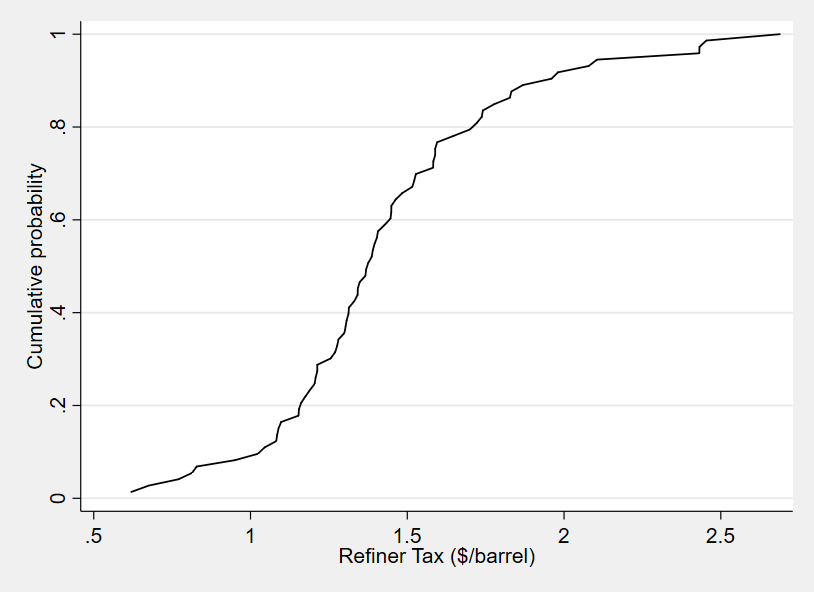
\includegraphics[width=0.48\textwidth]{\figpath/draft/mono_CO2TaxCDF_FP.png} \label{fig:taxCDF}}
  \hspace{5pt}%s
  \subfloat[Pass-through]{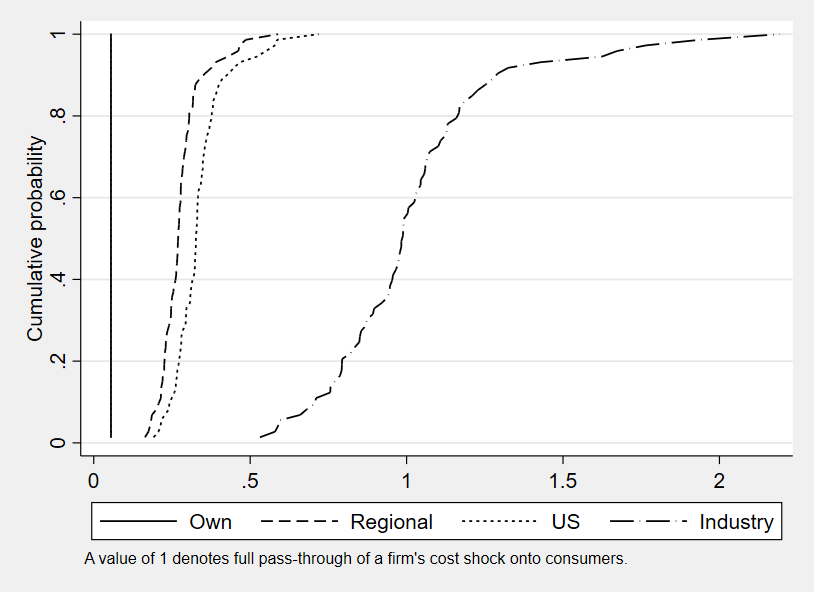
\includegraphics[width=0.48\textwidth]{\figpath/draft/mono_CO2Tax_PT_Allshocks.png} \label{fig:ghg_incidence}} \\
  \doublespacing
  Notes: Pass-through estimates in panel (b) based on model (5) of panel (b) in Table \ref{tab:RivalComp}.
\end{figure}

Heterogeneity in carbon intensity leads to dispersion in firm-level pass-through rates.  As was noted earlier when discussing equation (\ref{eq: MS_passthrough}), if a firm's closest rivals are more carbon-intensive, a tax provides the firm a competitive advantage, allowing the firm to pass-through a greater fraction of the tax.  In contrast, competition with less carbon-intensive rivals may discipline the firm's ability to pass-through the tax.

Figure \ref{fig:ghg_incidence} graphs the distribution of firm-level pass-through rates for the four policies described above. Under a tax that applies to a single firm (leftmost line), firm-level pass-through rates are identical, since rivals are unaffected.\footnote{Heterogeneity in pass-through may also arise from differences in regional demand or supply conditions. Tables that include interaction with firm size and HHI are not substantively different than our main results, and are provided in Appendix Table D.5.} Extending to a regional tax, firm-level pass-through rates begin to differ.  Some firms pass-through as little as 20 percent of their cost change, while others pass-though more than half.  Here, a carbon tax disadvantages carbon-intensive firms relative to less carbon-intensive rivals, limiting the ability of relatively carbon-intensive firms from passing-on the carbon tax.  Extending the tax to the national level increases the average pass-through rate, but also further increases the pass-through heterogeneity. Finally, the rightmost line presents the distribution using the full-pass through estimates across an domestic carbon tax, coupled with a commensurate border tax on imported fuels. Although consumers bear virtually all of the tax on average, firm-level pass-through rates vary substantially. Fifty-five percent of refineries pass-through the carbon tax less than fully, bearing some of the costs of the carbon tax.   But, the remaining 45 percent of refiners experience an \textit{increase} in markups under the tax.  Although the tax affects all firms, less carbon-intensive firms are competitively advantaged relative to more carbon-intensive rivals, allowing them to \emph{more than fully} pass on the carbon tax.  Such variation in firm-level pass-through rates is of direct political importance when considering whether particular firms might oppose (or support) such a policy.

\section{Conclusion\label{sec:Conclusion}}

Pass-through is an important tool with wide ranging economic applications. The extent to which prices change after a policy or event is also of paramount interest to policymakers. Due to its policy import and conceptual simplicity, pass-through is widely estimated. In this paper, we call attention to an underappreciated aspect of pass-through analysis:  strategic responses. In imperfectly competitive settings, the price a firm sets is a function of not just its own costs, but those of its rivals as well. Using a simple framework, we demonstrate that the link between the price a firm sets and competitor costs has important implications for estimation, interpretation and application of pass-through. These spillovers not only confound many standard research designs, but also they cannot simply be subsumed or ignored in estimation if the parameter of interest is the full response of prices to a common shock.

Using rich data from the U.S. oil refining industry, we demonstrate the empirical relevance of these points. We study the fracking boom, which upended the U.S. oil market and generated deep input cost discounts for some refineries but not others. Leveraging this shock, we demonstrate that firm prices do respond to competitor costs in practice, and that these own price adjustments vary intuitively with the proximity and scope of the shock. Comparing input cost shocks of different scope, our estimates of pass-through vary from near zero for firm-specific shocks to near one for shocks affecting all firms in the industry, reconciling seemingly disparate estimates of input cost pass-through from the literature.

Finally, we illustrate the benefit of explicitly considering indirect cost pass-through in the context of a hypothetical carbon tax on refinery emissions. Conditional on the direct effect on a firm's costs, the actual incidence borne varies dramatically depending on the extent to which that firm's rivals are taxed as well. Furthermore, we demonstrate that strategic spillovers generate large heterogeneity in pass-through across firms. This wide heterogeneity amongst firms may partially explain some of the intransigence of industry groups to carbon prices, despite the fact that the average incidence will fall primarily on consumers.


\clearpage

\bibliographystyle{aer}
\bibliography{MS_passthrough}

% UNCOMMENT THIS IF YOU USE ENDFLOAT
% PROCESS ALL FLOATS FROM MAIN TEXT BEFORE APPENDIX
\clearpage
%\processdelayedfloats
\clearpage


\end{document}
